\documentclass[12pt, a4paper]{article}
\usepackage[spanish]{babel}
\usepackage[utf8]{inputenc}
\usepackage[T1]{fontenc}
\usepackage{graphicx}
\usepackage{float}
\usepackage{enumitem}
\usepackage{booktabs}
\usepackage{array}
\usepackage{geometry}
\usepackage{helvet}
\usepackage{colortbl}
\usepackage{amssymb}
\usepackage{url}
\usepackage[12pt]{extsizes}
\usepackage{anyfontsize}
\usepackage{fancyhdr}
\usepackage{titlesec}
\usepackage{caption}
\usepackage{ragged2e} % Para justificacion avanzada
\usepackage{microtype} % Mejora la justificacion y el espaciado

% --- Configuracion de la pagina ---
\pagestyle{empty}
\geometry{
    a4paper,
    left=1.5cm,
    right=1.5cm,
    top=2cm,
    bottom=2cm,
}

% --- Fuentes y Colores ---
\renewcommand{\familydefault}{\sfdefault}
\definecolor{graycell}{RGB}{217, 217, 217}

% --- Formato de Titulos (segun plantilla) ---
\titleformat*{\section}{\fontsize{12}{14}\selectfont\bfseries}
\titleformat*{\subsection}{\fontsize{11}{13}\selectfont\bfseries}
\titleformat*{\subsubsection}{\fontsize{11}{13}\selectfont\bfseries\itshape}


\begin{document}

% --- Encabezado de la Practica ---
\begin{table}[H]
    \centering
    \arrayrulecolor{black}
    \setlength{\arrayrulewidth}{0.5pt}
    \renewcommand{\arraystretch}{1.5}
    \small
    \begin{tabular}{|p{3.4cm}|p{4.9cm}|p{2.0cm}|p{1.8cm}|p{2.0cm}|p{1.8cm}|}
    \hline
    \rowcolor{graycell}\textbf{DEPARTAMENTO:} & 
    \cellcolor{white}\textbf{CIENCIAS DE LA COMPUTACI\'ON} & 
    \textbf{CARRERA:} & 
    \multicolumn{3}{p{5.6cm}|}{\cellcolor{white}\textbf{INGENIER\'IA DE SOFTWARE}} \\
    \hline
    \rowcolor{graycell}\textbf{ASIGNATURA:} & 
    \cellcolor{white}Pruebas de Software & 
    \textbf{NIVEL:} & 
    \cellcolor{white}6to & 
    \cellcolor{graycell}\textbf{FECHA:} & 
    \cellcolor{white}09/08/2025 \\
    \hline
    \rowcolor{graycell}\textbf{DOCENTE:} & 
    \cellcolor{white}Ing. Luis Castillo, Mgtr. & 
    \textbf{PR\'ACTICA N°:} & 
    \cellcolor{white}2 & 
    \cellcolor{graycell}\textbf{CALIF.:} & 
    \cellcolor{white} \\
    \hline
    \end{tabular}
\end{table}
\vspace{1cm}

% --- Titulo (TL 14) ---
\begin{center}
    \fontsize{14}{16}\selectfont\textbf{CI/CD usando GitHub Actions}
\end{center}

% --- Nombre del Estudiante (TL 12) ---
\begin{center}
    \fontsize{12}{14}\selectfont\textbf{Yeshua Amador Chiliquinga Amaya}
    \vspace{0.5cm}
    \rule{\textwidth}{0.5pt}
\end{center}

% --- Resumen (TL 11) ---
\begin{center}
    \fontsize{11}{13}\selectfont\textbf{RESUMEN}
    \vspace{0.5cm}
    \parbox{0.9\textwidth}{\justifying
    En el presente laboratorio, se llev\'o a cabo la implementaci\'on de un flujo de trabajo de Integraci\'on Continua (CI) desde cero para un proyecto en Node.js. El proceso inici\'o con la configuraci\'on del entorno de desarrollo, incluyendo la instalaci\'on de dependencias clave como Jest para pruebas unitarias y ESLint para el an\'alisis est\'atico de c\'odigo. Posteriormente, se estableci\'o la comunicaci\'on con un repositorio remoto en GitHub. El n\'ucleo de la pr\'actica fue la creaci\'on y configuraci\'on de un workflow de GitHub Actions, dise\~nado para automatizar la ejecuci\'on de pruebas y la verificaci\'on de la calidad del c\'odigo con cada `push`. Se realizaron pruebas adicionales a\~nadiendo nuevas funcionalidades (factorial y Fibonacci) y se demostr\'o la efectividad del pipeline de CI al provocar un fallo intencionado, observar la notificaci\'on de error y, finalmente, corregirlo, validando as\'i el ciclo completo de detecci\'on y soluci\'on de problemas de forma automatizada.
    }
\end{center}
\vspace{0.5cm}

% --- Palabras Clave ---
\textbf{Palabras Claves:} GitHub Actions, Integraci\'on Continua, Jest.

\vspace{1cm}

% --- Secciones del Informe ---
\section*{1. INTRODUCCI\'ON}
La integraci\'on continua (CI) es una pr\'actica de desarrollo de software donde los desarrolladores fusionan sus cambios de c\'odigo en un repositorio central de forma frecuente. El prop\'osito de este laboratorio es familiarizarse con la automatizaci\'on de tareas esenciales como la instalaci\'on de dependencias, la ejecuci\'on de pruebas unitarias y la verificaci\'on de calidad del c\'odigo mediante ESLint, todo gestionado a trav\'es de GitHub Actions. A trav\'es de una aplicaci\'on sencilla en Node.js, se experimenta el poder de los flujos automatizados para detectar errores de forma temprana en el ciclo de vida del desarrollo.

\section*{2. OBJETIVOS}
\subsection*{2.1 Objetivo General}
Configurar un flujo de integraci\'on continua (CI) en GitHub Actions que se active autom\'aticamente con cada push a la rama principal del repositorio para automatizar la compilaci\'on y las pruebas del proyecto.

\subsection*{2.2 Objetivos Espec\'ificos}
\begin{itemize}
    \item Implementar pruebas unitarias usando Jest para garantizar que la l\'ogica del sistema funcione correctamente.
    \item Aplicar an\'alisis est\'atico de c\'odigo con ESLint para reforzar buenas pr\'acticas de programaci\'on.
    \item Observar y documentar el comportamiento del flujo de CI ante la introducci\'on de pruebas exitosas, fallidas y su posterior correcci\'on.
\end{itemize}

\section*{3. MARCO TE\'ORICO}
\subsection*{3.1 Entorno de Desarrollo}
\begin{itemize}
    \item \textbf{Node.js:} Entorno de ejecuci\'on de JavaScript del lado del servidor, que permite construir aplicaciones escalables.
    \item \textbf{Jest:} Un framework de pruebas de JavaScript, dise\~nado para garantizar la correcci\'on de cualquier base de c\'odigo JavaScript.
    \item \textbf{ESLint:} Herramienta de an\'alisis de c\'odigo est\'atico para identificar y reportar patrones problem\'aticos encontrados en el c\'odigo JavaScript.
    \item \textbf{GitHub Actions:} Plataforma de automatizaci\'on que permite construir, probar y desplegar c\'odigo directamente desde GitHub.
\end{itemize}

\section*{4. DESCRIPCI\'ON DEL PROCEDIMIENTO}
El laboratorio comenz\'o con la inicializaci\'on de un proyecto de Node.js y la configuraci\'on del entorno de desarrollo. Se utiliz\'o el comando \texttt{npm install jest eslint --save-dev} para instalar Jest y ESLint como dependencias de desarrollo, lo cual es una buena pr\'actica para mantener separadas las librer\'ias necesarias para la producci\'on de las que solo se usan para pruebas y an\'alisis (Figura \ref{fig:install_jest}). A continuaci\'on, se crearon los archivos base del proyecto: \texttt{sum.js} para la l\'ogica de negocio inicial, y \texttt{sum.test.js} para su prueba unitaria correspondiente, estableciendo las bases para un desarrollo guiado por pruebas (Figura \ref{fig:archivos_creados}).

\begin{figure}[H]
    \centering
    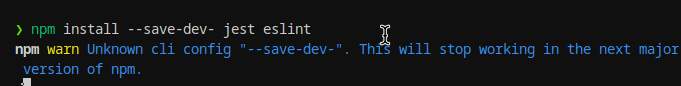
\includegraphics[width=0.8\textwidth]{img/instalar modo desarrollo jest eslint.png}
    \caption{Instalaci\'on de Jest y ESLint como dependencias de desarrollo.}
    \label{fig:install_jest}
\end{figure}

\begin{figure}[H]
    \centering
    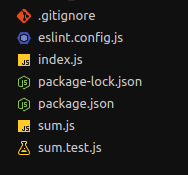
\includegraphics[width=0.5\textwidth]{img/todos los archivos creados.png}
    \caption{Estructura de archivos inicial del proyecto.}
    \label{fig:archivos_creados}
\end{figure}

Para gestionar las tareas del proyecto, se modific\'o el archivo \texttt{package.json}. Se definieron scripts clave como \texttt{test} para ejecutar Jest y \texttt{lint} para ejecutar ESLint. Adem\'as, se a\~nadi\'o la directiva \texttt{"type": "module"} para habilitar el uso de m\'odulos ES6 (import/export), modernizando la base del c\'odigo (Figura \ref{fig:package_json}). Se configur\'o tambi\'en un archivo \texttt{.gitignore} para excluir la carpeta \texttt{node\_modules} del control de versiones, evitando as\'i subir al repositorio las dependencias que pueden ser instaladas en cualquier entorno con \texttt{npm install} (Figura \ref{fig:gitignore}).

\begin{figure}[H]
    \centering
    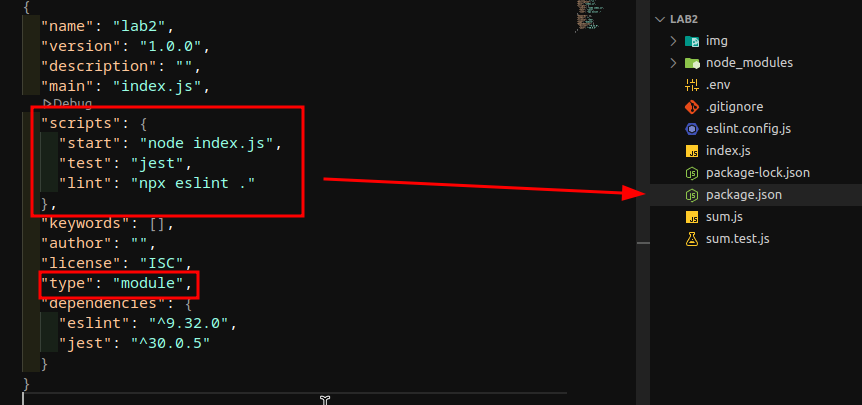
\includegraphics[width=0.6\textwidth]{img/dentro de package json la configuracion de start lint test y type module.png}
    \caption{Configuraci\'on de scripts y tipo de m\'odulo en package.json.}
    \label{fig:package_json}
\end{figure}

\begin{figure}[H]
    \centering
    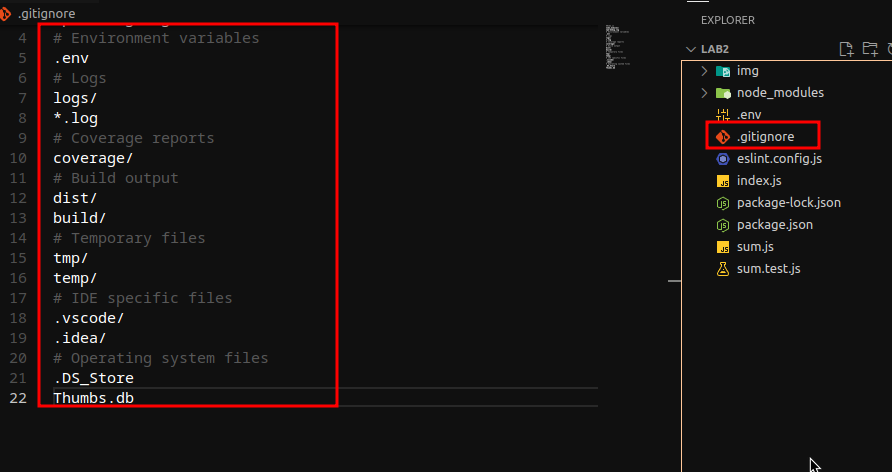
\includegraphics[width=0.65\textwidth]{img/configuracion gitignore.png}
    \caption{Configuraci\'on del archivo .gitignore.}
    \label{fig:gitignore}
\end{figure}

Con el proyecto configurado localmente, el siguiente paso fue establecer el repositorio remoto en GitHub. Se cre\'o un nuevo repositorio vac\'io (Figura \ref{fig:repo_vacio}) y se ejecut\'o la secuencia de comandos \texttt{git init}, \texttt{git add .}, \texttt{git commit}, \texttt{git branch}, \texttt{git remote add} y \texttt{git push} para enlazar el proyecto local y subir los archivos por primera vez (Figuras \ref{fig:git_push} y \ref{fig:repo_actualizado}).

\begin{figure}[H]
    \centering
    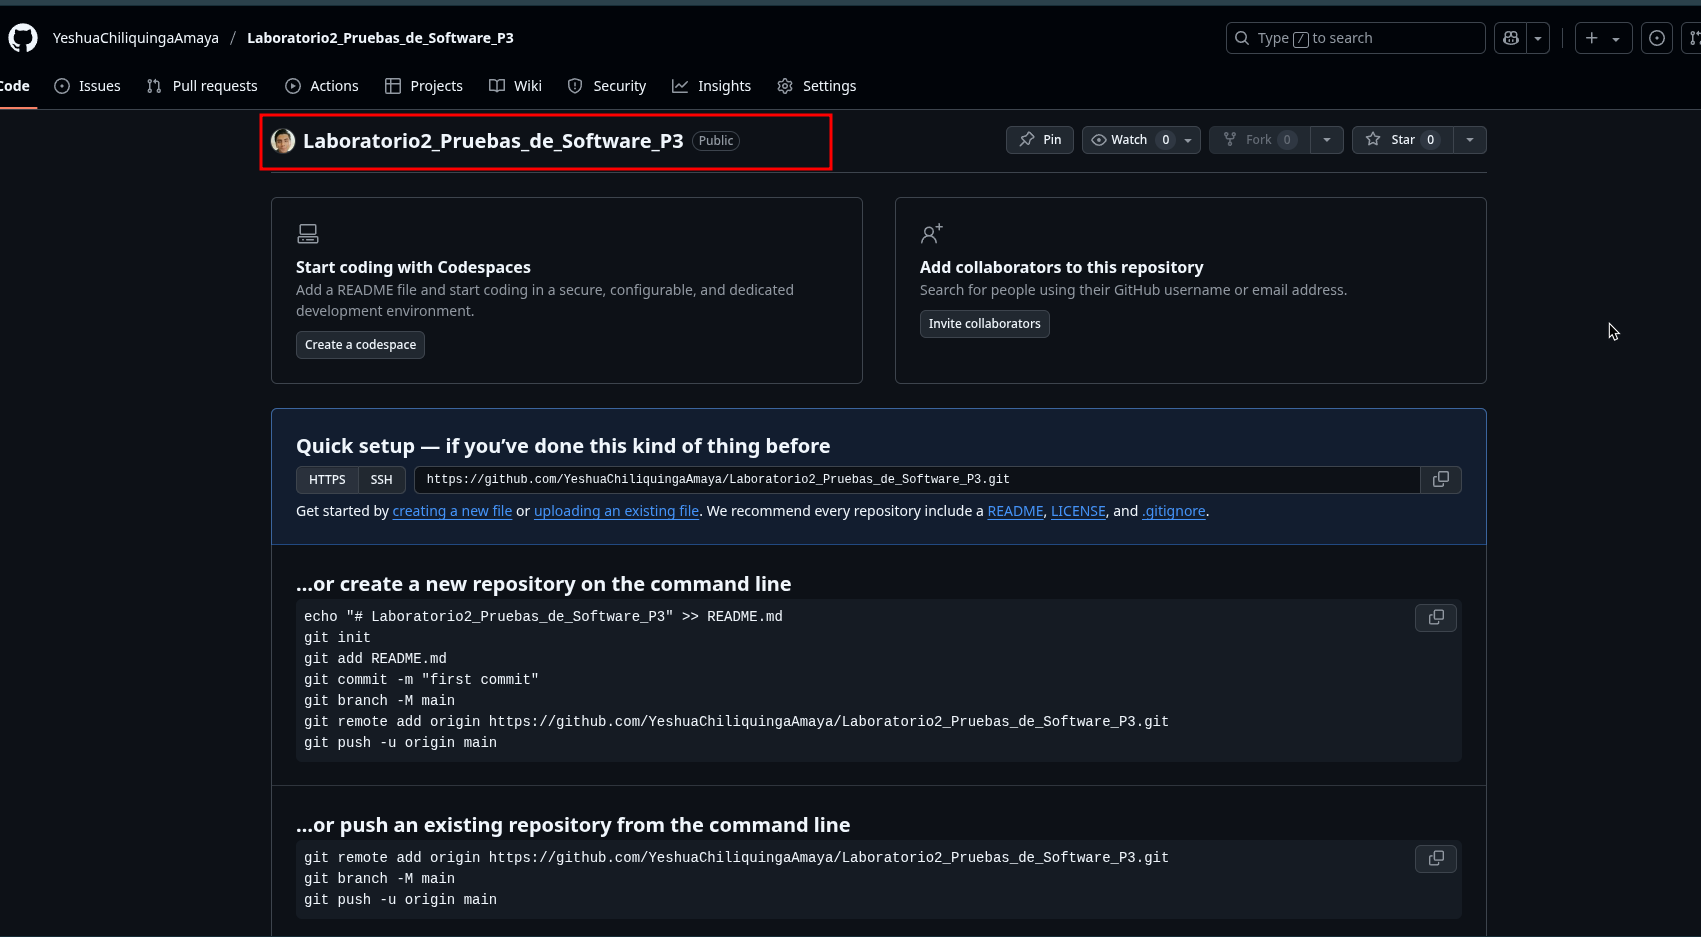
\includegraphics[width=0.9\textwidth]{img/creamos repositorio en github vacio.png}
    \caption{Creaci\'on del repositorio vac\'io en GitHub.}
    \label{fig:repo_vacio}
\end{figure}

\begin{figure}[H]
    \centering
    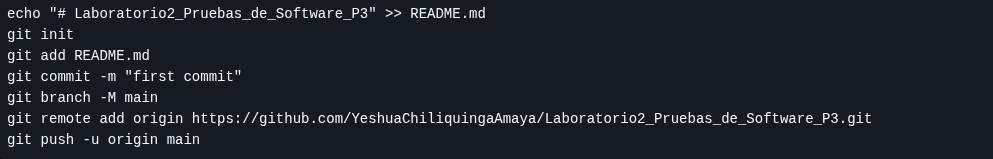
\includegraphics[width=0.6\textwidth]{img/pasos necesrios para poder guardar los archivos locales dentro de github desde echo init add commit branch remoteadd push.png}
    \caption{Comandos para subir el proyecto local a GitHub.}
    \label{fig:git_push}
\end{figure}

\begin{figure}[H]
    \centering
    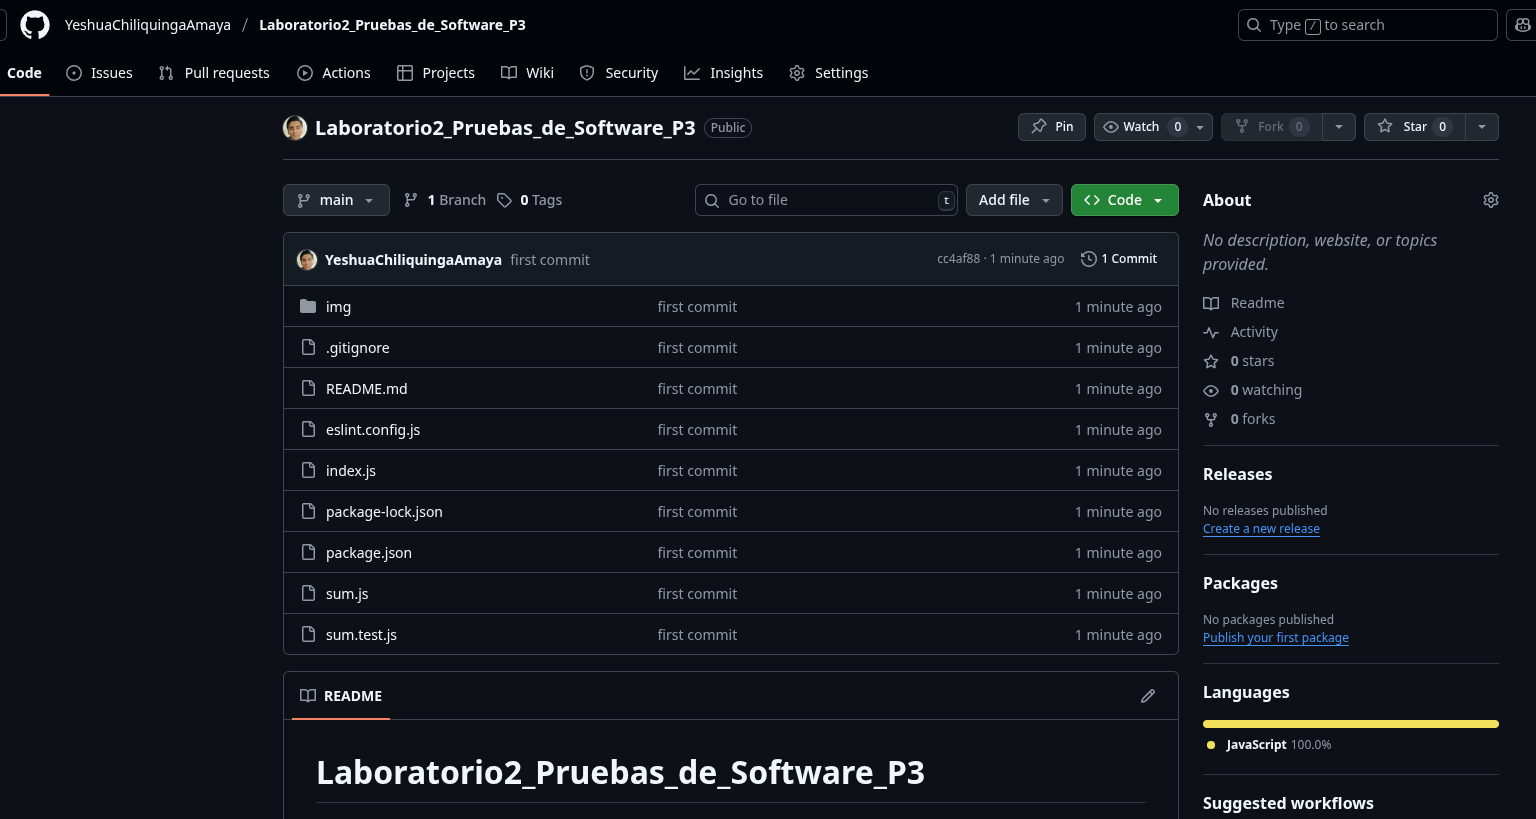
\includegraphics[width=0.9\textwidth]{img/si hicimos correctamete ya veriamos el repo de github actualizado.png}
    \caption{Verificaci\'on del repositorio actualizado en GitHub.}
    \label{fig:repo_actualizado}
\end{figure}

Finalmente, se implement\'o el flujo de CI. Se cre\'o la estructura de carpetas \texttt{.github/workflows} y dentro de ella el archivo \texttt{ci.yml} (Figura \ref{fig:crear_ci_yml}). En este archivo se defini\'o el pipeline: se especific\'o que se activara con cada `push` a la rama `main`, que utilizara un entorno de Node.js v20, y que ejecutara secuencialmente los pasos de `checkout` del c\'odigo, instalaci\'on de dependencias con \texttt{npm ci}, an\'alisis de c\'odigo con \texttt{npm run lint} y ejecuci\'on de pruebas con \texttt{npm run test} (Figura \ref{fig:config_ci_yml}). Al hacer `push` de este nuevo archivo, GitHub Actions detect\'o el workflow y lo ejecut\'o autom\'aticamente. El resultado fue un \'exito, indicado por una marca de verificaci\'on verde, confirmando que la configuraci\'on inicial era correcta y el pipeline funcional (Figura \ref{fig:workflow_verde}).

\begin{figure}[H]
    \centering
    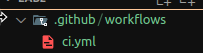
\includegraphics[width=0.9\textwidth]{img/creamos ciyml dnetro de github y workflows.png}
    \caption{Creaci\'on del archivo de configuraci\'on del workflow.}
    \label{fig:crear_ci_yml}
\end{figure}

\begin{figure}[H]
    \centering
    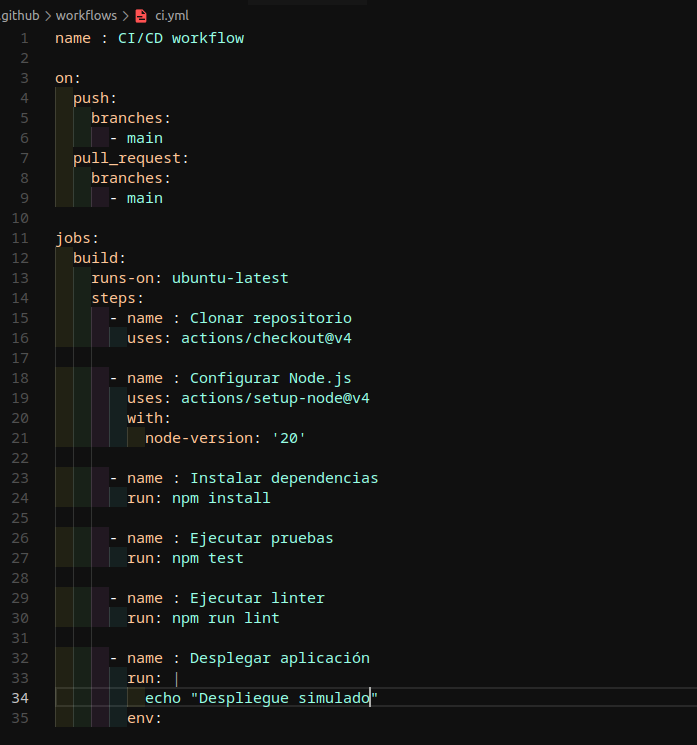
\includegraphics[width=0.65\textwidth]{img/configuracion inicial de ciyml en la cual se maneja todo lo necesrio para el despliegue.png}
    \caption{Contenido del archivo ci.yml con los pasos del workflow.}
    \label{fig:config_ci_yml}
\end{figure}

\begin{figure}[H]
    \centering
    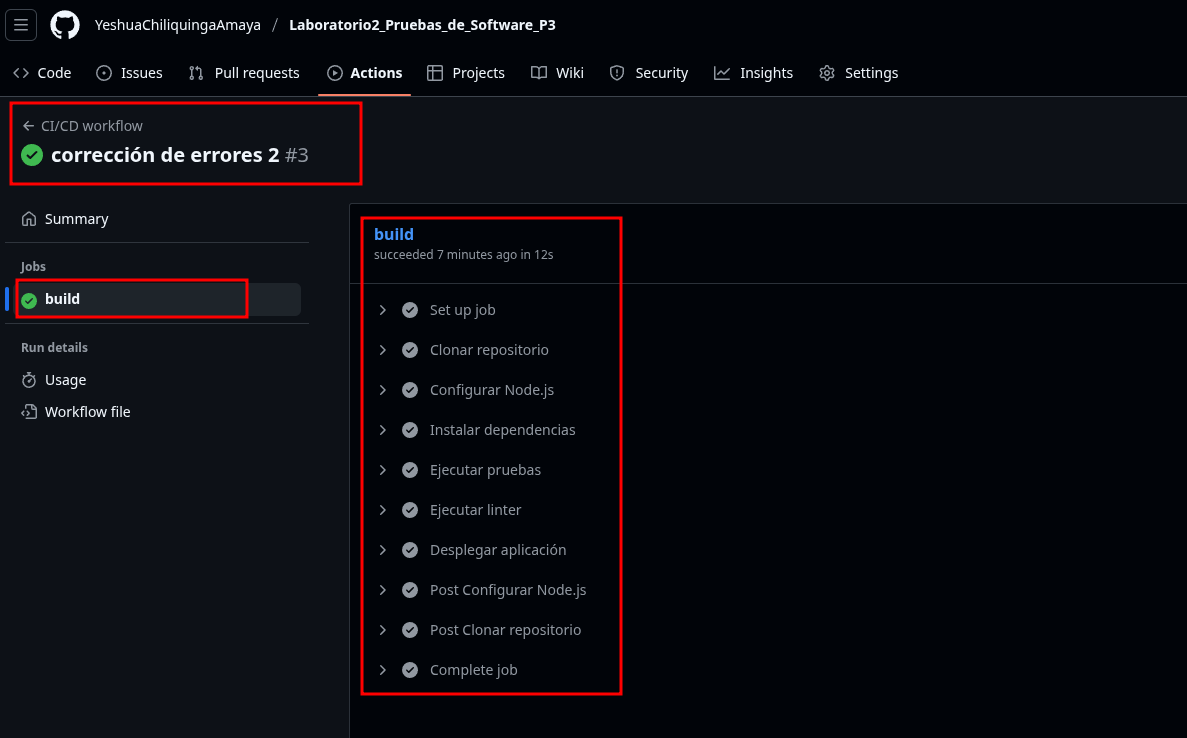
\includegraphics[width=0.9\textwidth]{img/podemos ver el flujo de trabajo en verde indicando que todo salio correctamente pero si sale en rojo podemos identificar que algo fallo en algunas de las pruebas.png}
    \caption{Flujo de trabajo ejecutado exitosamente en GitHub Actions.}
    \label{fig:workflow_verde}
\end{figure}

\section*{5. PREGUNTAS/ACTIVIDADES}
Para validar la extensibilidad del proyecto y la robustez del pipeline, se procedi\'o a a\~nadir nueva funcionalidad. Se implementaron dos funciones matem\'aticas cl\'asicas, factorial y Fibonacci, en el archivo \texttt{math.js} (Figuras \ref{fig:func_factorial} y \ref{fig:func_fibonacci}). Siguiendo las buenas pr\'acticas, para cada nueva funci\'on se crearon sus correspondientes pruebas unitarias en un nuevo archivo \texttt{math.test.js}. Estas pruebas cubr\'ian casos base y casos t\'ipicos para asegurar que la l\'ogica implementada era correcta (Figura \ref{fig:pruebas_math}). Al realizar el `push` con estas nuevas adiciones, el flujo de trabajo de CI en GitHub Actions se dispar\'o autom\'aticamente. El pipeline ejecut\'o todos los pasos definidos, incluyendo las nuevas pruebas, y concluy\'o exitosamente, lo que se visualiz\'o con un build en verde. Esto demostr\'o que las nuevas funcionalidades estaban correctamente implementadas y no romp\'ian ninguna parte existente del c\'odigo (Figura \ref{fig:build_verde}).

\begin{figure}[H]
    \centering
    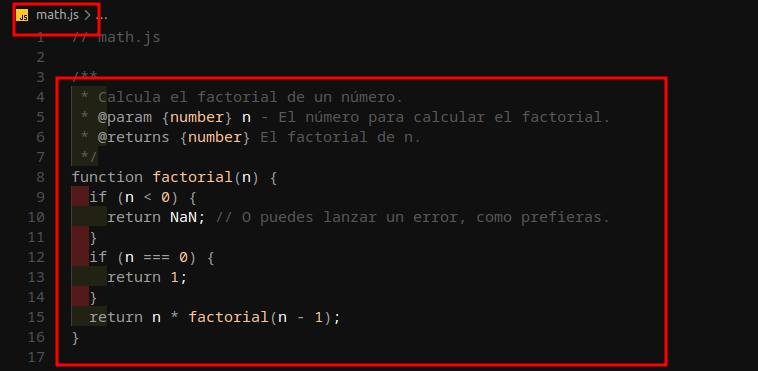
\includegraphics[width=0.7\textwidth]{img/nueva funcion en mathjs la de factorial.png}
    \caption{Funci\'on de factorial a\~nadida en math.js.}
    \label{fig:func_factorial}
\end{figure}

\begin{figure}[H]
    \centering
    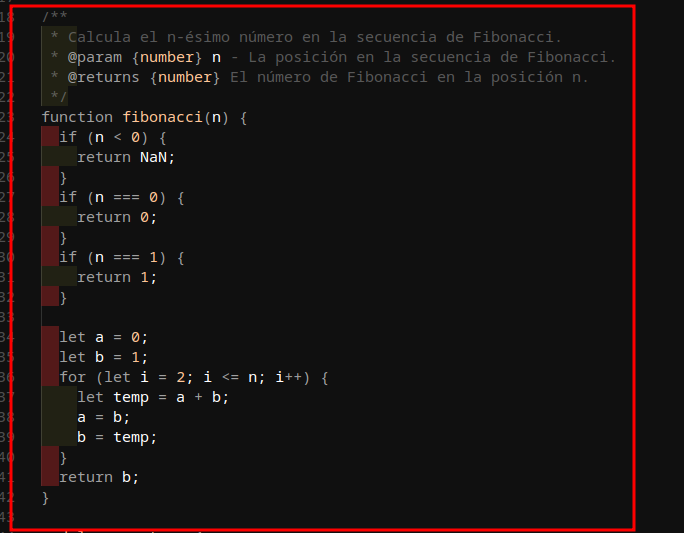
\includegraphics[width=0.7\textwidth]{img/nueva funcion fibonacci en mathjs.png}
    \caption{Funci\'on de Fibonacci a\~nadida en math.js.}
    \label{fig:func_fibonacci}
\end{figure}

\begin{figure}[H]
    \centering
    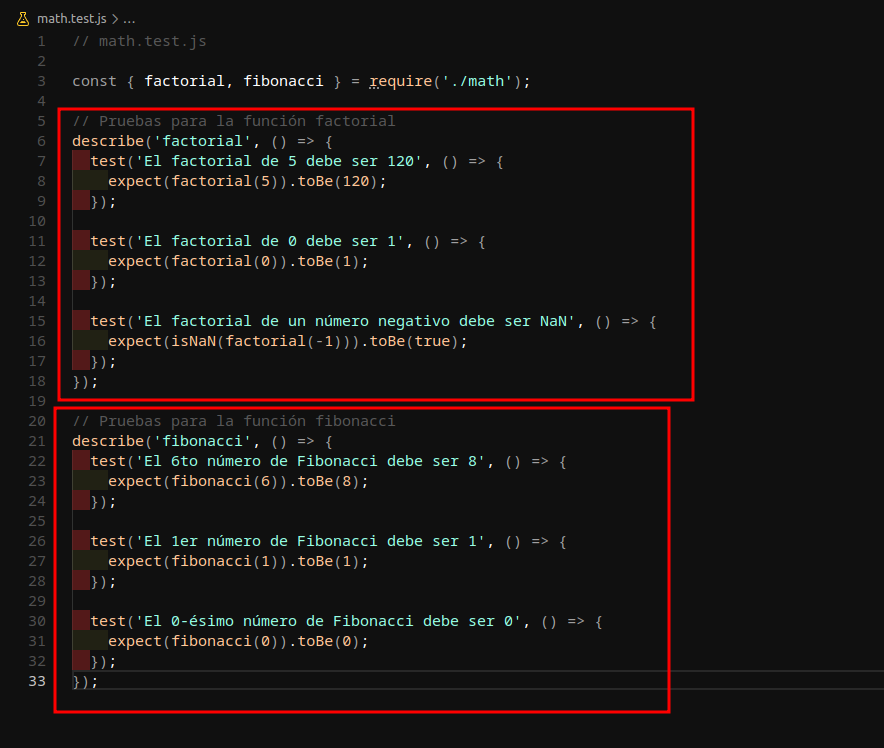
\includegraphics[width=0.9\textwidth]{img/respectivas pruebas para fibonacci y para factaorial en el math testjs.png}
    \caption{Pruebas unitarias para factorial y Fibonacci en math.test.js.}
    \label{fig:pruebas_math}
\end{figure}

\begin{figure}[H]
    \centering
    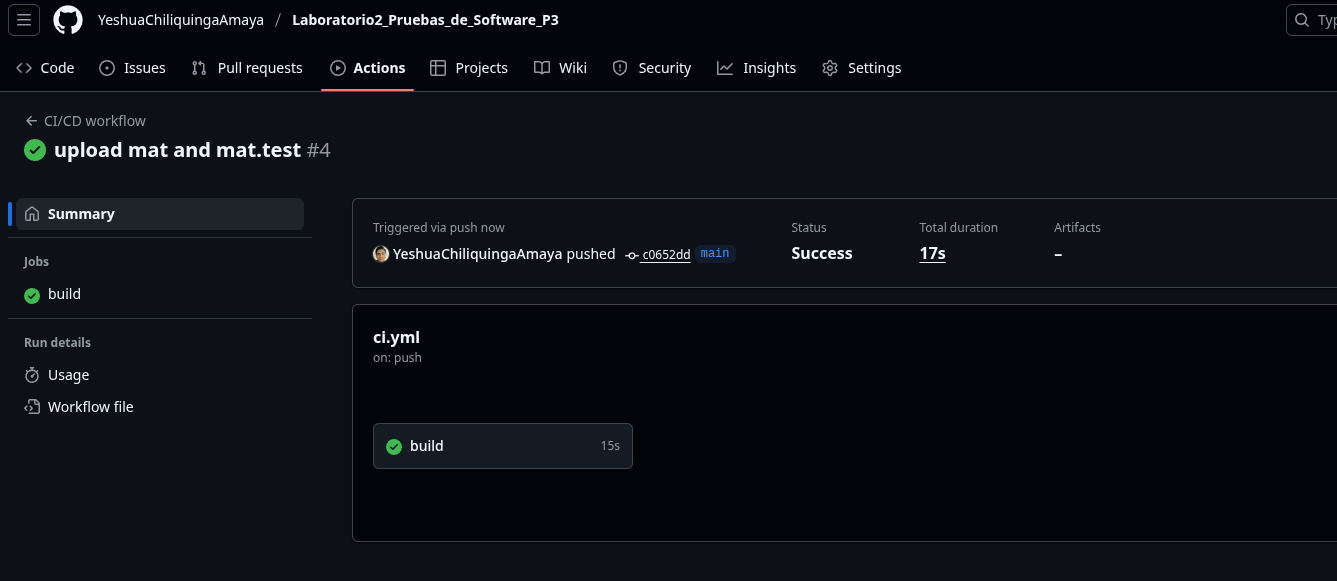
\includegraphics[width=0.9\textwidth]{img/salo todo bien en mattestjs sallio con visto verde y build.png}
    \caption{El build en GitHub Actions se completa con \'exito tras a\~nadir las nuevas pruebas.}
    \label{fig:build_verde}
\end{figure}

El siguiente paso fue simular un escenario real de desarrollo: la introducci\'on de un error. Se modific\'o intencionadamente el archivo \texttt{sum.test.js} para que una prueba fallara; se cambi\'o la aserci\'on de que `2 + 3` es `5` a que es `100` (Figura \ref{fig:error_intencional}). Inmediatamente despu\'es de hacer `push` de este cambio, GitHub Actions inici\'o el pipeline y, como era de esperar, fall\'o en el paso de ejecuci\'on de pruebas. La interfaz de GitHub mostr\'o una "X" roja junto al commit, indicando visualmente el fallo. Al hacer clic en los detalles, se pod\'ia ver exactamente qu\'e prueba hab\'ia fallado y el motivo, proporcionando una retroalimentaci\'on r\'apida y precisa sobre el origen del problema (Figura \ref{fig:workflow_rojo}).

\begin{figure}[H]
    \centering
    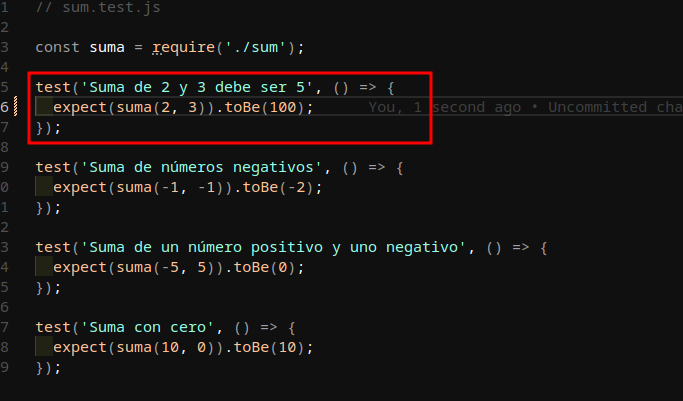
\includegraphics[width=0.7\textwidth]{img/configuramos sumtestjs para que falle haciendo que la suma de 2 y 3 sea 100 y por ende de error.png}
    \caption{Modificaci\'on de sum.test.js para provocar un fallo intencional.}
    \label{fig:error_intencional}
\end{figure}

\begin{figure}[H]
    \centering
    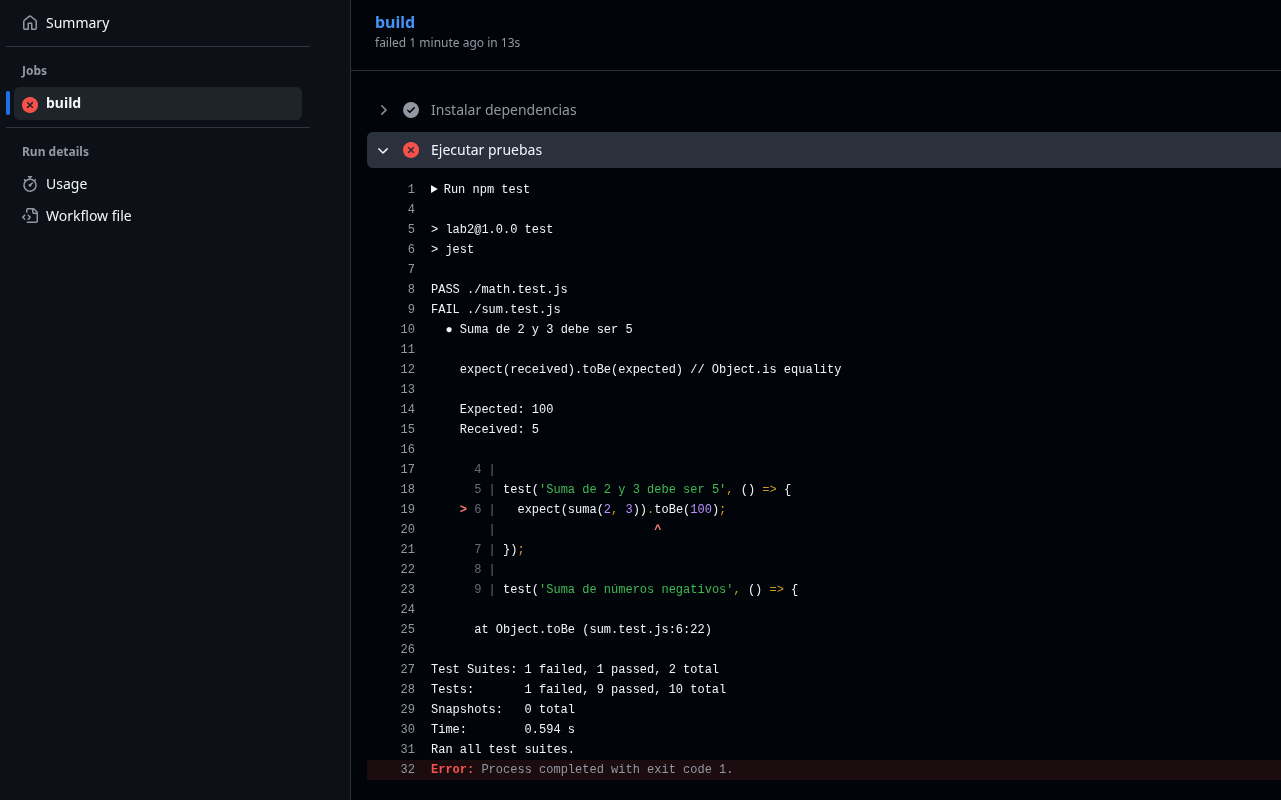
\includegraphics[width=0.9\textwidth]{img/el codigo fallo y en github podemos ver en donde y que linea nos da el error para poder corregir y por ende nos da una x en color rojo de error.png}
    \caption{El flujo de CI falla y GitHub Actions reporta el error.}
    \label{fig:workflow_rojo}
\end{figure}

Finalmente, se complet\'o el ciclo de detecci\'on y correcci\'on. Se revirti\'o el cambio en \texttt{sum.test.js} a su estado original y correcto, donde la suma de `2 + 3` esperaba el resultado `5` (Figura \ref{fig:codigo_corregido}). Tras confirmar y subir la correcci\'on con un nuevo `push`, el pipeline de CI se ejecut\'o una vez m\'as. Esta vez, todas las pruebas pasaron, el linter no report\'o problemas y el flujo de trabajo se complet\'o con \'exito, mostrando nuevamente la marca de verificaci\'on verde (Figura \ref{fig:workflow_verde_final}). Este proceso valid\'o la efectividad del pipeline de CI como una red de seguridad que previene la integraci\'on de c\'odigo defectuoso en la rama principal.

\begin{figure}[H]
    \centering
    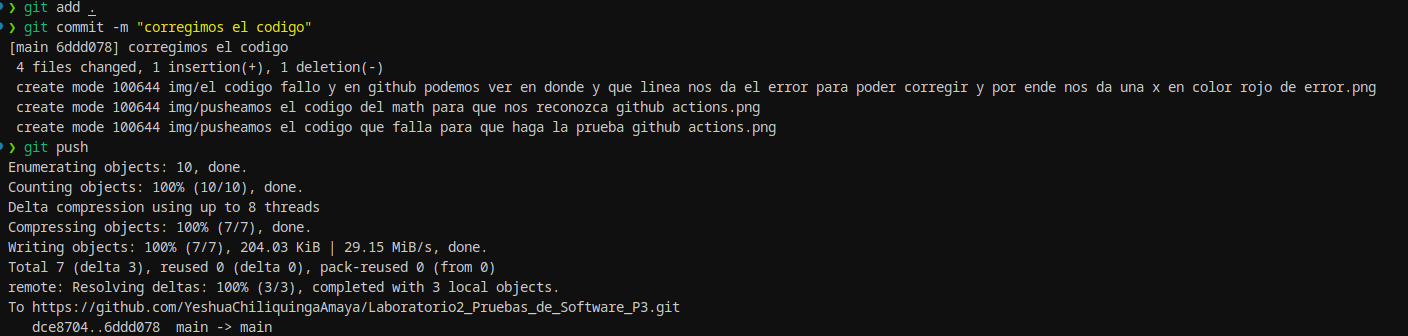
\includegraphics[width=0.8\textwidth]{img/corregimos el codigo para que nos reconozca github actions con el codigo bien hecho.png}
    \caption{Correcci\'on del c\'odigo en el archivo de prueba.}
    \label{fig:codigo_corregido}
\end{figure}

\begin{figure}[H]
    \centering
    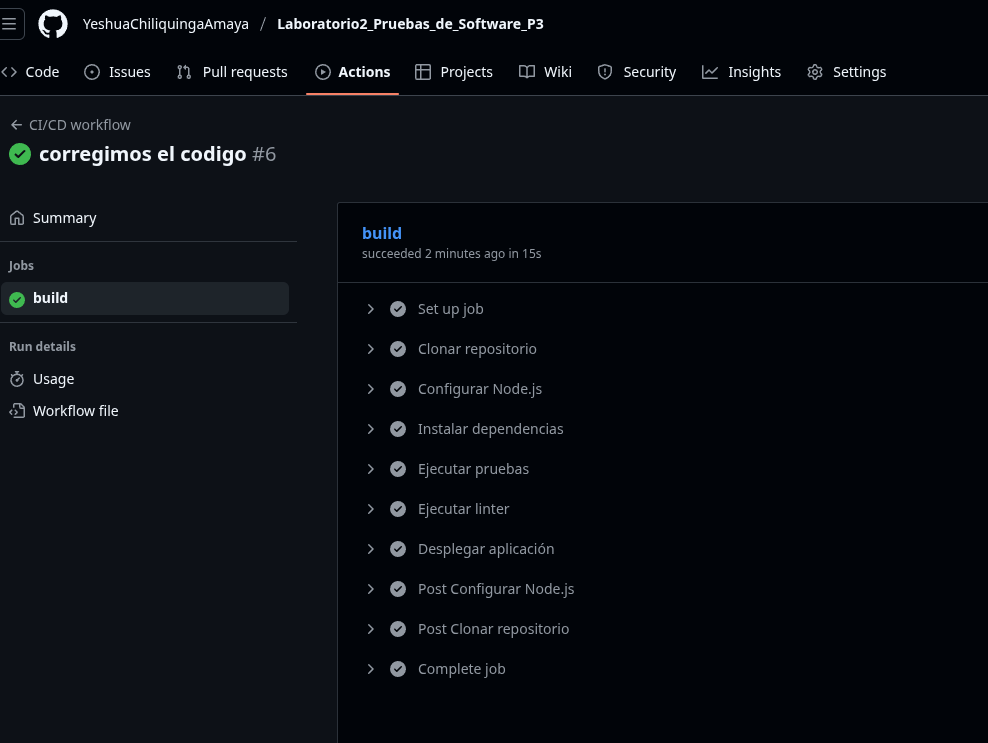
\includegraphics[width=0.9\textwidth]{img/en github acitons vemos que esta todo correcto y nos salto en verde.png}
    \caption{El flujo de trabajo vuelve a ser exitoso tras la correcci\'on.}
    \label{fig:workflow_verde_final}
\end{figure}

\section*{6. CONCLUSIONES}
\begin{itemize}[leftmargin=*]
    \item La implementaci\'on de un flujo de Integraci\'on Continua con GitHub Actions es una herramienta eficaz para automatizar la validaci\'on del c\'odigo, asegurando que cada cambio cumpla con los est\'andares de calidad y funcionalidad definidos antes de ser fusionado.
    \item La retroalimentaci\'on inmediata que proporciona el pipeline de CI es fundamental. La capacidad de detectar errores al instante mediante notificaciones visuales (rojo/verde) permite a los desarrolladores corregirlos r\'apidamente, evitando que los problemas se integren en la rama principal y afecten a otros miembros del equipo.
    \item El uso de un archivo de configuraci\'on como \texttt{ci.yml} estandariza el entorno de pruebas y validaci\'on. Esto garantiza que el c\'odigo se eval\'ue siempre de la misma manera (misma versi\'on de Node.js, mismas dependencias, mismos comandos), eliminando el cl\'asico problema de ``en mi m\'aquina funciona'' y asegurando la consistencia en todo el ciclo de desarrollo.
\end{itemize}

\section*{7. RECOMENDACIONES}
\begin{itemize}[leftmargin=*]
    \item Es recomendable separar los trabajos (\texttt{jobs}) en el archivo de workflow si las tareas son independientes (p. ej., un job para linting y otro para pruebas) para optimizar el tiempo de ejecuci\'on al permitir que se ejecuten en paralelo, lo que puede reducir significativamente el tiempo de espera para obtener retroalimentaci\'on.
    \item Utilizar secretos de GitHub (`GitHub Secrets`) para manejar credenciales, tokens o claves de API en lugar de escribirlas directamente en el archivo \texttt{.yml}. Esta pr\'actica es crucial para mejorar la seguridad del proyecto y evitar la exposici\'on accidental de informaci\'on sensible en el repositorio de c\'odigo.
    \item Implementar el almacenamiento en cach\'e de dependencias (\texttt{caching}) dentro del workflow de GitHub Actions. Para proyectos con muchas dependencias, como los de Node.js, guardar en cach\'e la carpeta \texttt{node\_modules} puede acelerar dr\'asticamente las ejecuciones posteriores del pipeline, ya que se evita tener que descargar e instalar todas las librer\'ias desde cero en cada ejecuci\'on.
\end{itemize}

\section*{8. BIBLIOGRAF\'IA}
\noindent\hangindent=1.5em
[1] GitHub, ``GitHub Actions Documentation'', 2025. [En l\'inea]. Disponible: \url{https://docs.github.com/en/actions}

\noindent\hangindent=1.5em
[2] Jest, ``Jest - Delightful JavaScript Testing'', 2025. [En l\'inea]. Disponible: \url{https://jestjs.io/}

\end{document}
